%-----------------------------------------------------------------------------%
\chapter{\babTiga}
%-----------------------------------------------------------------------------%
%\todo{tambahkan kata-kata pengantar bab 1 disini}
Penelitian ini bertujuan untuk mengevaluasi konfigurasi Hypervisor KVM yang disediakan secara langsung dalam konteks penggunaan \vm\ pada Apache Cloudstack. Tujuan utama adalah untuk memastikan bahwa \vm\ dapat mencapai kinerja yang optimal sesuai dengan spesifikasi sistem yang digunakan. Untuk mencapai tujuan ini, \saya akan melakukan penyesuaian konfigurasi atau tuning pada Hypervisor KVM dan kemudian membandingkannya dengan kondisi awal yang tidak mengalami tuning. Hasil pengujian akan dianalisis untuk menentukan apakah ada perbedaan signifikan dalam kinerja antara Hypervisor KVM yang telah dituning dengan yang belum dituning.

%-----------------------------------------------------------------------------%
\section{Tahapan Penelitian}
%-----------------------------------------------------------------------------%
\begin{figure}
	\centering
	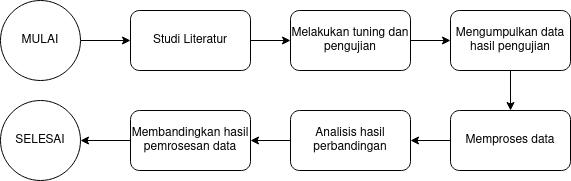
\includegraphics[width=1\textwidth]
	{assets/pics/tahapan-penelitian.png}
	\caption{Tahapan Penelitian}
	\label{fig:TahapanPenelitian}
\end{figure}

Penelitian ini akan dilakukan dalam beberapa tahap sesuai dengan diagram di gambar \ref{fig:TahapanPenelitian}. Tahap pertama melibatkan studi literatur untuk mengumpulkan semua informasi yang diperlukan untuk penelitian ini. Studi literatur ini penting karena memberikan dasar pengetahuan yang kuat tentang topik yang akan diteliti, memungkinkan \saya untuk memahami konteks dan kerangka kerja yang relevan.

Selanjutnya, penelitian melibatkan tuning terhadap Hypervisor KVM dan pengujian dilakukan dengan mengkompresi video menggunakan aplikasi Handbrake. Pengujian dengan Handbrake bertujuan untuk mengukur efisiensi dan kinerja Hypervisor KVM setelah tuning. Hasil pengujian Handbrake ini akan digunakan untuk membandingkan waktu kompresi video antara Hypervisor KVM yang tidak dituning dengan yang sudah dituning. Hasil dari perbandingan ini akan memberikan gambaran mengenai konfigurasi yang paling optimal dan sesuai, serta membantu dalam pemahaman lebih lanjut tentang pengaruh tuning terhadap performa Hypervisor KVM dalam konteks kompresi video.

%-----------------------------------------------------------------------------%
\section{Persiapan Lingkungan untuk Pengujian dan Analisis}
%-----------------------------------------------------------------------------%
\begin{figure}
	\centering
	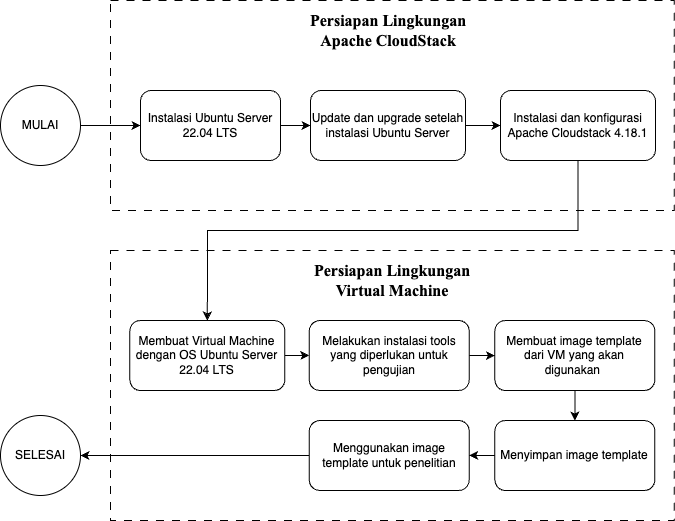
\includegraphics[width=1\textwidth]
	{assets/pics/persiapan_lingkungan_penelitian.png}
	\caption{PersiapanLingkunganPenelitian}
	\label{fig:PersiapanLingkunganPenelitian}
\end{figure}


Proses persiapan lingkungan untuk pengujian dan analisis yang tergambar dalam gambar \ref{fig:PersiapanLingkunganPenelitian} menggambarkan serangkaian langkah sistematis yang penting untuk memastikan integritas hasil penelitian. Proses ini dimulai dengan tahap inisiasi yang meliputi instalasi Ubuntu Server 22.04 LTS, sebuah sistem operasi yang stabil dan sering digunakan untuk keperluan server. Instalasi ini menjadi landasan dasar bagi infrastruktur yang akan dikembangkan.

Setelah sistem operasi terinstal, dilakukan pembaruan dan peningkatan sistem operasi tersebut untuk memastikan semua komponen sistem berada pada versi terkini serta keamanan sistem terjaga. Langkah ini krusial untuk menutup potensi kerentanan yang mungkin ada pada sistem. Selanjutnya, Apache Cloudstack versi 4.18.1 diinstal dan dikonfigurasi. Apache Cloudstack berfungsi sebagai platform manajemen cloud yang memungkinkan pembuatan dan pengelolaan infrastruktur cloud yang kompleks, yang merupakan elemen kunci dalam penelitian ini.

Dalam pembuatan lingkungan virtual, dibuat \vm yang menggunakan sistem operasi yang sama, yaitu Ubuntu Server 22.04 LTS. Pembuatan VM ini memungkinkan simulasi berbagai skenario penelitian dalam lingkungan yang terisolasi. Selanjutnya, untuk keperluan analisis dan pengujian, Handbrake diinstal, dan video yang akan digunakan pun disiapkan.

Tahapan selanjutnya merupakan pembuatan image template dari VM yang telah dikonfigurasi. Proses ini memungkinkan duplikasi VM dengan cepat dan efisien untuk pengujian berulang atau skenario analisis yang berbeda, menjamin konsistensi lingkungan penelitian. Image template ini kemudian digunakan sebagai standar untuk penelitian lebih lanjut, memastikan bahwa setiap VM yang dibuat untuk tujuan pengujian memiliki konfigurasi yang identik.

Setelah semua dilakukan hal ini menandakan bahwa lingkungan penelitian telah siap untuk diuji dan dianalisis. Kesiapan lingkungan ini esensial untuk memastikan bahwa pengujian yang dilakukan dapat diulang dan hasilnya valid.

%-----------------------------------------------------------------------------%
\section{Tuning Hypervisor KVM}
%-----------------------------------------------------------------------------%
Tuning Hypervisor KVM yang dilakukan adalah dengan menambahkan flag instruksi yang tidak terdapat pada konfigurasi KVM default, dimana flag default dari KVM yang mendukung kompresi video hanyalah sse, dan sse2.

\begin{figure}
	\begin{alltt}
		\textbf{fpu} vme \textbf{de pse tsc msr pae mce cx8 apic sep mtrr pge mca} 
		\textbf{cmov pat pse36 clflush mmx fxsr sse sse2} ht \textbf{syscall nx} 
		mmxext fxsr_opt pdpe1gb rdtscp \textbf{lm} constant_tsc \textbf{rep_good} acc_power
		\textbf{nopl} nonstop_tsc \textbf{cpuid}  \textbf{extd_apicid} aperfmperf \textbf{pni} pclmulqdq 
		monitor ssse3 fma \textbf{cx16} sse4_1  sse4_2 movbe popcnt aes xsave avx 
		f16c \textbf{lahf_lm} cmp_legacy \textbf{svm} extapic cr8_legacy abm sse4a misalignsse
		\textbf{3dnowprefetch} osvw ibs xop skinit wdt lwp fma4 tce nodeid_msr tbm
		topoext perfctr_core perfctr_nb bpext ptsc mwaitx cpb hw_pstate ssbd 
		\textbf{vmmcall} fsgsbase bmi1 avx2 smep bmi2 xsaveopt arat npt lbrv svm_lock
		nrip_save tsc_scale vmcb_clean flushbyasid decodeassists pausefilter 
		pfthreshold avic v_vmsave_vmload vgif overflow_recov
	\end{alltt}
	\caption{Seluruh flag instruksi di Host}
	\label{fig:flag_kvm_host}
\end{figure}

Terlihat pada gambar \ref{fig:flag_kvm_host} adalah keseluruhan flag instruksi dari sistem host, sedangkan text yang ditajamkan adalah flag instruksi bawaan default dari hypervisor KVM. Dari sini flag yang berguna untuk melakukan kompresi video dan ditajamkan hanyalah sse dan sse2, hal ini menandakan bahwa KVM tidak mengaktifkan keseluruhan flag instruksi meskipun pada sistem host sudah mendukung flag instruksinya. Beberapa flag yang berguna untuk melakukan kompresi video dan tidak dinyalakan oleh hypervisor KVM adalah SSE3, SSE4\_1, dan SSE4\_2. 

\saya\ dapat mengaktifkan flag tersebut untuk digunakan oleh \vm\ yang menggunakan hypervisor KVM. Untuk melakukan tuning \saya\ dapat menggunakan tools virsh untuk mengubah konfigurasi \vm dari CloudStack. Secara default konfigurasi dari \vm di CloudStack akan seperti ini:

\begin{listing}[H]
	\begin{minted}{xml}
		<domain type='kvm'>
		
			...
			
			<cpu mode='custom' match='exact' check='full'>
				<model fallback='forbid'>qemu64</model>
				<feature policy='require' name='x2apic'/>
				<feature policy='require' name='hypervisor'/>
				<feature policy='require' name='lahf_lm'/>
			</cpu>
			
			...
			
		</domain>
	\end{minted}
	\caption{Konfigurasi default dari KVM}
	\label{code:default_kvm_xml}
\end{listing}

Terlihat dari kode \ref{code:default_kvm_xml} bahwa feature yang dinyalakan tidak memuat sse3, sse4\_1, dan sse4\_2. Untuk itu \saya\ dapat menambahkan fitur tersebut sehingga \vm dapat menggunakan flag instruksi tersebut. Perubahahan yang akan \saya lakukan akan seperti ini:

\begin{listing}[H]
	\begin{minted}{xml}
		<domain type='kvm'>
		
			...
			
			<cpu mode='custom' match='exact' check='full'>
				<model fallback='forbid'>qemu64</model>
				<feature policy='require' name='x2apic'/>
				<feature policy='require' name='hypervisor'/>
				<feature policy='require' name='lahf_lm'/>
				<feature policy='require' name='sse3'/>
				<feature policy='require' name='sse4_1'/>
				<feature policy='require' name='sse4_2'/>
			</cpu>
			
			...
			
		</domain>
	\end{minted}
	\caption{Konfigurasi tuning KVM}
	\label{code:tuned_kvm_xml}
\end{listing}

Jika sudah dilakukan penambahan fitur seperti di kode \ref{code:tuned_kvm_xml} sekarang \vm yang menggunakan Hypervisor KVM sudah bisa mendukung set instruksi tersebut.

%-----------------------------------------------------------------------------%
\section{Pengujian Kompresi Video Dengan HandBrake}
%-----------------------------------------------------------------------------%
Untuk menguji dan membandingkan kinerja Hypervisor KVM sebelum dan sesudah tuning, {\saya} akan menggunakan software HandBrake, sebuah software kompresi video yang sudah banyak digunakan. Proses ini melibatkan penggunaan HandBrake untuk kompresi video pada dua lingkungan \vm\ yang berbeda, yang mana satu menggunakan KVM yang belum di-tuning dan yang lainnya menggunakan KVM yang telah di-tuning. Tujuan dari pengujian ini adalah untuk mengevaluasi sejauh mana tuning Hypervisor KVM dapat mempengaruhi kecepatan kompresi video.

HandBrake dipilih karena kemampuannya yang baik dalam mengkompresi video dan mudah untuk digunakan\cite{Folgar2014eg}. Dalam pengujian ini, video yang akan digunakan adalah "COSTA RICA IN 4K 60fps HDR (ULTRA HD)" yang diunduh dari YouTube dengan resolusi video yang digunakan adalah 2K. Video ini dipilih karena resolusi tingginya, yang memberikan tantangan yang baik untuk menguji efisiensi kompresi video pada kedua lingkungan \vm. 

Parameter penting yang akan diukur dalam pengujian ini adalah: 

\begin{enumerate}
	\item \textbf{\f{Time Elapsed}}
	
	\f{Time Elapsed} atau berapa lama waktu yang dibutuhkan oleh masing-masing \vm\ untuk menyelesaikan proses kompresi video.
		
	\item \textbf{\f{Structural Similarity Index Measure Score}}
	
	Structural Similarity Index Measure adalah cara untuk menilai kesamaan dari 2 buah gambar, untuk melihat apakah terjadi penurunan kualitas atau perbedaan yang besar antara gambar yang belum di compress dengan gambar yang sudah di compress.
\end{enumerate}


Data ini yang akan memberikan gambaran yang jelas mengenai perbedaan kinerja antara KVM yang telah di-tuning dengan yang belum.

Spesifikasi dari \vm\ yang akan digunakan dalam pengujian ini adalah sebagai berikut:
\begin{itemize}
	\item \textbf{Cloud Platform}: Apache CloudStack 4.18.1
	\item \textbf{OS}: Ubuntu Server 22.04 LTS
	\item \textbf{CPU}: 1 CPU x 1.00 Ghz
	\item \textbf{Memory}: 1024 MB
\end{itemize} 

Perintah yang digunakan untuk melakukan kompresi video dengan handbrake adalah sebagai berikut:

\begin{verbatim}
	./HandBrakeCLI -i /path/to/input.mov -o /path/to/output.mp4
	-e x264 -q 28 -r 15 -B 64 -X 1280 -O
\end{verbatim}

Dengan perintah ini \saya akan melakukan kompresi video dengan codec x264. Codec yang dikembangkan oleh VideoLAN yang sudah banyak digunakan dikarenakan mampu untuk melakukan kompresi video yang baik dan rendahnya tingkat penurunan kualitas gambar.

%-----------------------------------------------------------------------------%
\section{Analisis Pengujian}
%-----------------------------------------------------------------------------%
Dalam analisis ini, waktu kompresi untuk Hypervisor KVM yang belum di-tuning akan disebut sebagai $T_{\mathrm{default}}$, sementara waktu kompresi untuk Hypervisor KVM yang telah di-tuning akan disebut sebagai $T_{\mathrm{tuned}}$. Waktu kompresi ini akan diambil dari logs HandBrake yang telah melakukan kompresi video. Untuk mengetahui apakah terdapat perbedaan yang signifikan, \saya\ dapat menggunakan formula speedup. 

\[ \mathrm{Speedup} = \frac{T_{\mathrm{default}}}{T_{\mathrm{tuned}}} \]

Jika nilai speedup lebih dari 1, ini menandakan bahwa proses kompresi dengan Hypervisor KVM yang sudah di-tuning lebih cepat dibandingkan dengan yang belum di-tuning. 

Pengujian akan dilakukan sebanyak kurang lebih sepuluh kali dan nantinya akan ditampilkan dalam bentuk grafik. Akan terdapat grafik \f{line chart} dengan dua garis dimana masing-merepresentasikan $T_{\mathrm{default}}$ dan $T_{\mathrm{tuned}}$.

Selain menganalisis waktu kompresi video, \saya\ juga akan melakukan analisis untuk menilai kualitas video yang telah dikompresi. Analisis ini akan melibatkan perbandingan nilai dari \f{Structural Similarity Index Measure} (SSIM) antara video yang dikompres menggunakan Hypervisor KVM default dan Hypervisor KVM yang telah di-tuning. SSIM adalah metrik yang mengukur kesamaan visual antara dua video. Semakin tinggi nilai SSIM, semakin mirip video yang dikompres dengan versi aslinya. Oleh karena itu, nilai SSIM yang lebih tinggi menunjukkan kualitas kompresi yang lebih baik, dimana integritas visual dari video asli lebih terjaga.


\iffalse
Selanjutnya, \saya\ akan menghitung efisiensi dari tuning Hypervisor KVM ini. Untuk mengetahui efisiensi, \saya\ dapat menggunakan formula efisiensi.

\[ \mathrm{Efficiency} = \frac{\mathrm{Speedup}}{\frac{R_{\mathrm{tuned}}}{R_{\mathrm{default}}}} \]


Tujuan menghitung efisiensi ini adalah untuk mengetahui seberapa efektif tuning dilakukan dalam menggunakan sumber daya yang ada, seperti penggunaan CPU dan memori. Perhitungan ini penting untuk menilai kinerja tuning dalam konteks keseluruhan penggunaan sumber daya, tidak hanya kecepatan kompresi.
\fi

% Time Measurement
%$T_{\mathrm{default}}$, $T_{\mathrm{tuned}}$
%\[ T_{\mathrm{default}}, \quad T_{\mathrm{tuned}} \]

% Speedup
%$\mathrm{Speedup} = \frac{T_{\mathrm{default}}}{T_{\mathrm{tuned}}}$
%\[ \mathrm{Speedup} = \frac{T_{\mathrm{default}}}{T_{\mathrm{tuned}}} \]



\iffalse
%-----------------------------------------------------------------------------%
\section{Satu Persamaan}
%-----------------------------------------------------------------------------%

\noindent \begin{align}\label{eq:garis}
	\cfrac{y - y_{1}}{y_{2} - y_{1}} = 
	\cfrac{x - x_{1}}{x_{2} - x_{1}}
\end{align}

\equ~\ref{eq:garis} diatas adalah persamaan garis. 
\equ~\ref{eq:garis} dan \ref{eq:bola} sama-sama dibuat dengan perintah \bslash
align. 
Perintah ini juga dapat digunakan untuk menulis lebih dari satu persamaan. 

\noindent \begin{align}\label{eq:bola}
	\underbrace{|\overline{ab}|}_{\text{pada bola $|\overline{ab}| = r$}} 
	= \sqrt[2]{(x_{b} - x_{a})^{2} + (y_{b} - y_{a})^{2} + 
		\vert\vert(z_{b} - z_{a})^{2}}
\end{align}

%-----------------------------------------------------------------------------%
\section{Lebih dari Satu Persamaan}
\label{sec:multiEqu}
%-----------------------------------------------------------------------------%
\noindent \begin{align}\label{eq:matriks}	
	|\overline{a} * \overline{b}| &= |\overline{a}| |\overline{b}| \sin\theta 
	\\[0.2cm]
	\overline{a} * \overline{b} &=  
	\begin{array}{| c c c |}
		\hat{i} & x_{1} & x_{2} \\
		\hat{j} & y_{1} & y_{2} \\
		\hat{k} & z_{1} & z_{2} \\
	\end{array} \nonumber \\[0.2cm]
	&= \hat{i} \,
	\begin{array}{ | c c | }
		y_{1} & y_{2} \\
		z_{1} & z_{2} \\
	\end{array} 
	+ \hat{j} \,
	\begin{array}{ | c c | }
		z_{1} & z_{2} \\
		x_{1} & x_{2} \\
	\end{array} 
	+ \hat{k} \,	
	\begin{array}{ | c c | }
		x_{1} & x_{2} \\
		y_{1} & y_{2} \\
	\end{array}
	\nonumber
\end{align}

Pada \equ~\ref{eq:matriks} dapat dilihat beberapa baris menjadi satu bagian 
dari \equ~\ref{eq:matriks}. 
Sedangkan dibawah ini dapat dilihat bahwa dengan cara yang sama, \equ~
\ref{eq:gabungan1}, \ref{eq:gabungan2}, dan \ref{eq:gabungan3} memiliki nomor 
persamaannya masing-masing. 

\noindent \begin{align}\label{eq:gabungan1}	
	\int_{a}^{b} f(x)\, dx + \int_{b}^{c} f(x) \, dx = \int_{a}^{c} f(x) \, dx
	\\\label{eq:gabungan2}
	\lim_{x \to \infty} \frac{f(x)}{g(x)} = 0 \hspace{1cm} 
	\text{jika pangkat $f(x)$ $<$ pangkat $g(x)$} \\\label{eq:gabungan3}
	a^{m^{a \, ^{n}\log b }} = b^{\frac{m}{n}}
\end{align}
\fi
